%%%%%%%%%%%%%%%%%%%%%%%%%%%%%%%%%%%%%%%%%
% Classicthesis-Styled CV
% LaTeX Template
% Version 1.0 (22/2/13)
%
% This template has been downloaded from:
% http://www.LaTeXTemplates.com
%
% Original author:
% Alessandro Plasmati
%
% License:
% CC BY-NC-SA 3.0 (http://creativecommons.org/licenses/by-nc-sa/3.0/)
%
%%%%%%%%%%%%%%%%%%%%%%%%%%%%%%%%%%%%%%%%%

%----------------------------------------------------------------------------------------
%	PACKAGES AND OTHER DOCUMENT CONFIGURATIONS
%----------------------------------------------------------------------------------------

\documentclass{scrartcl}

\reversemarginpar % Move the margin to the left of the page 

\newcommand{\MarginText}[1]{\marginpar{\raggedleft\itshape\small#1}} % New command defining the margin text style

\usepackage{graphicx}
\usepackage[nochapters]{classicthesis} % Use the classicthesis style for the style of the document
\usepackage[LabelsAligned]{currvita} % Use the currvita style for the layout of the document

\renewcommand{\cvheadingfont}{\LARGE\color{Maroon}} % Font color of your name at the top

\usepackage{hyperref} % Required for adding links	and customizing them
\hypersetup{colorlinks, breaklinks, urlcolor=Maroon, linkcolor=Maroon} % Set link colors

\newlength{\datebox}\settowidth{\datebox}{Spring 201111} % Set the width of the date box in each block

\newcommand{\NewEntry}[3]{\noindent\hangindent=2em\hangafter=0 \parbox{\datebox}{\small \textit{#1}}\hspace{1.5em} #2 #3 % Define a command for each new block - change spacing and font sizes here: #1 is the left margin, #2 is the italic date field and #3 is the position/employer/location field
\vspace{0.5em}} % Add some white space after each new entry

\newcommand{\Description}[1]{\hangindent=2em\hangafter=0\noindent\raggedright\footnotesize{#1}\par\normalsize\vspace{1em}} % Define a command for descriptions of each entry - change spacing and font sizes here

\pagenumbering{gobble}
%----------------------------------------------------------------------------------------

\begin{document}

\thispagestyle{empty} % Stop the page count at the bottom of the first page

%----------------------------------------------------------------------------------------
%	NAME AND CONTACT INFORMATION SECTION
%----------------------------------------------------------------------------------------

\begin{cv}{\spacedallcaps{Damar Canggih Wicaksono}}\vspace{1.5em} % Your name

\noindent\spacedlowsmallcaps{Personal Information}\vspace{0.5em} % Personal information heading

\NewEntry{}{\textit{Born in Jakarta,}}{15 May 1986} % Birthplace and date

\NewEntry{email}{\href{mailto:damar.wicaksono@gmail.com}{damar.wicaksono@gmail.com.com}} % Email address

\NewEntry{GitHub}{\href{https://github.com/damar-wicaksono}{https://github.com/damar-wicaksono}} % Personal website

\NewEntry{phone}{(M) +41 (0) 78 798 5785} % Phone number(s)

\smash{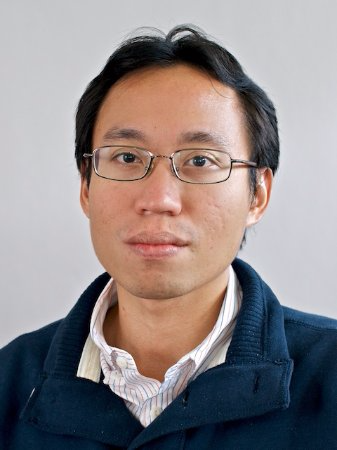
\includegraphics[width=2.35cm]{wd41_photo}}
%\noindent\spacedlowsmallcaps{Goal}\vspace{1em} % Goal heading, could be used for a quotation or short profile instead

%\Description{Gain fundamental experience in my area of interest and expertise.}\vspace{2em} % Goal text

\vspace{2em} % Extra white space between the personal information section and goal

%----------------------------------------------------------------------------------------
%	EDUCATION
%----------------------------------------------------------------------------------------

%\includegraphics[width=3cm]{M02-z33v}
\spacedlowsmallcaps{Education}\vspace{1em}

\NewEntry{2013-2018}{EPF Lausanne, Switzerland}

\Description{\MarginText{Doctor of Science}\textit{Nuclear Engineering}\newline 
Thesis: \textit{Bayesian Uncertainty Quantification of Physical Models in Thermal-Hydraulics System Codes}\newline
Description: This thesis explored the idea that money has been the cause of untold anguish and suffering in the world. I found that it has, in fact, not.\newline
Advisors: Prof.~James \textsc{Smith} \& Assoc. Prof.~Jane \textsc{Smith}}

%------------------------------------------------

\NewEntry{2010-2012}{EPF Lausanne -- ETH Z\"urich, Switzerland}

\Description{\MarginText{Master of Science}\textit{Nuclear Engineering}\ \ $\cdotp$\ \ GPA: 5.52/6.00\newline 
Thesis: \textit{Development}\newline
Description: This thesis explored the idea that money has been the cause of untold anguish and suffering in the world. I found that it has, in fact, not.\newline
Advisors: Prof.~James \textsc{Smith} \& Assoc. Prof.~Jane \textsc{Smith}}

%------------------------------------------------

\NewEntry{2004-2009}{Universitas Gadjah Mada, Indonesia}

\Description{\MarginText{Bachelor of Engineering}\textit{Nuclear Engineering}\ \ $\cdotp$\ \ GPA: 3.92/4.00\ \ $\cdotp$\ \ \textit{Cum Laude Graduate}\newline
Description: This degree focussed heavily on important things such as personnel management and mundane paperwork.}

%------------------------------------------------

\vspace{1em} % Extra space between major sections

%----------------------------------------------------------------------------------------
%	WORK EXPERIENCE
%----------------------------------------------------------------------------------------

\noindent\spacedlowsmallcaps{Work Experience}\vspace{1em}

\NewEntry{2013--2018}{Doctoral Assistant}

\Description{\MarginText{Paul Scherrer Institut / EPF Lausanne}Developed spreadsheets for risk analysis on exotic derivatives on a wide array of commodities (ags, oils, precious and base metals), managed blotter and secondary trades on structured notes, liaised with Middle Office, Sales and Structuring for bookkeeping. \\ Reference: John \textsc{McDonald}\ \ $\cdotp$\ \ +1 (000) 111 1111\ \ $\cdotp$\ \ \href{mailto:john@lehman.com}{john@lehman.com}}

%------------------------------------------------

\NewEntry{Aug-Nov 2011}{Intern}

\Description{\MarginText{Paul Scherrer Institut}Rated "truly distinctive" for Analytical Skills and Teamwork. \\ Reference: Bill \textsc{Lumbergh}\ \ +1 (000) 111 1111\ \ $\cdotp$\ \ \href{mailto:bill@initech.com}{bill@initech.com}}

%------------------------------------------------

\NewEntry{Jul-Oct 2011}{Intern}

\Description{\MarginText{Kernkraftwerk Leibstadt AG}Worked in the Nerd Herd and helped to solve computer problems by asking customers to turn their computers off and on again. \\ Reference: Big \textsc{Mike}\ \ +1 (000) 111 1111\ \ $\cdotp$\ \ \href{mailto:mike@buymore.com}{mike@buymore.com}}

%------------------------------------------------

\vspace{1em} % Extra space between major sections

\clearpage
%----------------------------------------------------------------------------------------
%	PUBLICATIONS
%----------------------------------------------------------------------------------------

\spacedlowsmallcaps{Publications and Conference Contributions}\vspace{1em}

\Description{D. Wicaksono, O. Zerkak, and A. Pautz, ``Global Sensitivity Analysis of Transient Code Output applied to a Reflood Experiment Model using TRACE Code,'' \textit{Nuclear Science and Engineering}, vol. 184, no. 6, 2016.}

%------------------------------------------------

\Description{D. Wicaksono, O. Zerkak, and A. Pautz, ``Bayesian Caliration of Thermal-Hydraulics Model with Time-Dependent Output,'' in the \textit{11th International Topical Meeting on Nuclear Thermal-Hydraulics, Operation and Safety (NUTHOS-11)}, Gyeongju, South Korea, Oct. 9--13, 2016.}

%------------------------------------------------

\Description{D. Wicaksono, O. Zerkak, and A. Pautz, ``A Methodology for Global Sensitivity Analysis of Transient Code Output applied to a Reflood Experiment Model using TRACE,'' in the \textit{16th International Topical Meeting on Nuclear Reactor Thermal-Hydraulics}, Chicago, Illinois, Aug. 30 -- Sept. 4, 2015.}

%------------------------------------------------

\Description{D. Wicaksono, O. Zerkak, and A. Pautz, ``Sensitivity Analysis of a Bottom Reflood Simulation using the Morris Screening Method,'' in the \textit{10th International Topical Meeting on Nuclear Thermal-Hydraulics, Operation and Safety (NUTHOS-10)}, Okinawa, Japan, Dec. 14 -- 18, 2014.}

%------------------------------------------------

\Description{D. Wicaksono, O. Zerkak, and A. Pautz, ``Exploring Variability in Reflood Simulation Results: an Application of Functional Data Analysis,'' in the \textit{10th International Topical Meeting on Nuclear Thermal-Hydraulics, Operation and Safety (NUTHOS-10)}, Okinawa, Japan, Dec. 14 -- 18, 2014.}

%------------------------------------------------

\vspace{1em} % Extra space between major sections

%----------------------------------------------------------------------------------------
%	COMPUTER SKILLS
%----------------------------------------------------------------------------------------

\spacedlowsmallcaps{Computer Skills}\vspace{1em}

\Description{\MarginText{Basic}\textsc{java}, Adobe Illustrator}

\Description{\MarginText{Intermediate}\textsc{python}, \textsc{html}, \LaTeX, OpenOffice, Linux, Microsoft Windows}

\Description{\MarginText{Advanced}Computer Hardware and Support}

%------------------------------------------------

\vspace{1em} % Extra space between major sections

%----------------------------------------------------------------------------------------
%	OTHER INFORMATION
%----------------------------------------------------------------------------------------

\spacedlowsmallcaps{Awards and Accolades}\vspace{1em}

\Description{2015\ \ $\cdotp$\ \ Best Student Paper \ \ $\cdotp$ \ \ NURETH-16, American Nuclear Society}

\vspace{-0.5em} % Negative vertical space to counteract the vertical space between every \Description command

\Description{2014\ \ $\cdotp$\ \ Best Student Paper \ \ $\cdotp$ \ \ NUTHOS-11, Japanese Nuclear Society}

\vspace{-0.5em} % Negative vertical space to counteract the vertical space between every \Description command

\Description{2014\ \ $\cdotp$\ \ Best 1st Graduate Student \ \ $\cdotp$ \ \ NES PhD Day, Paul Scherrer Institut}

\vspace{-0.5em} % Negative vertical space to counteract the vertical space between every \Description command

\Description{2010-2012\ \ $\cdotp$\ \ Excellence Scholarship\ \ $\cdotp$ \ \ Federal Commission for Scholarship, Switzerland}

\vspace{-0.5em} % Negative vertical space to counteract the vertical space between every \Description command

\Description{2009\ \ $\cdotp$\ \ Cum Laude Graduate\ \ $\cdotp$ \ \ Universitas Gadjah Mada, Indonesia}

%------------------------------------------------

\vspace{1em}

\newlength{\langbox} % Create a new length for the length of languages to keep them equally spaced
\settowidth{\langbox}{Indonesian} % Length equals the length of "English" - if you have a longer language in your list put it here

\Description{\MarginText{Languages}\parbox{\langbox}{\textsc{Indonesian}}\ \ $\cdotp$\ \ \ Mothertongue}

\vspace{-0.5em} % Negative vertical space to counteract the vertical space between every \Description command

\Description{\parbox{\langbox}{\textsc{English}}\ \ $\cdotp$\ \ \ Professional fluency}

\vspace{-0.5em} % Negative vertical space to counteract the vertical space between every \Description command

\Description{\parbox{\langbox}{\textsc{French}}\ \ $\cdotp$\ \ \ Intermediate (B1)}

\vspace{-0.5em} % Negative vertical space to counteract the vertical space between every \Description command

\Description{\parbox{\langbox}{\textsc{German}}\ \ $\cdotp$\ \ \ Basic (A1.2)}

\vspace{1em} % Negative vertical space to counteract the vertical space between every \Description command

%------------------------------------------------

\Description{\MarginText{Interests}Reading\ \ $\cdotp$\ \ Cooking\ \ $\cdotp$\ \ Hiking\ \ $\cdotp$\ \ Coding}

%----------------------------------------------------------------------------------------

\end{cv}

\end{document}